
\section{Insegnante}
\subsection{UC 2.1 Visualizza profilo personale}

\begin{figure}[H]
\centering
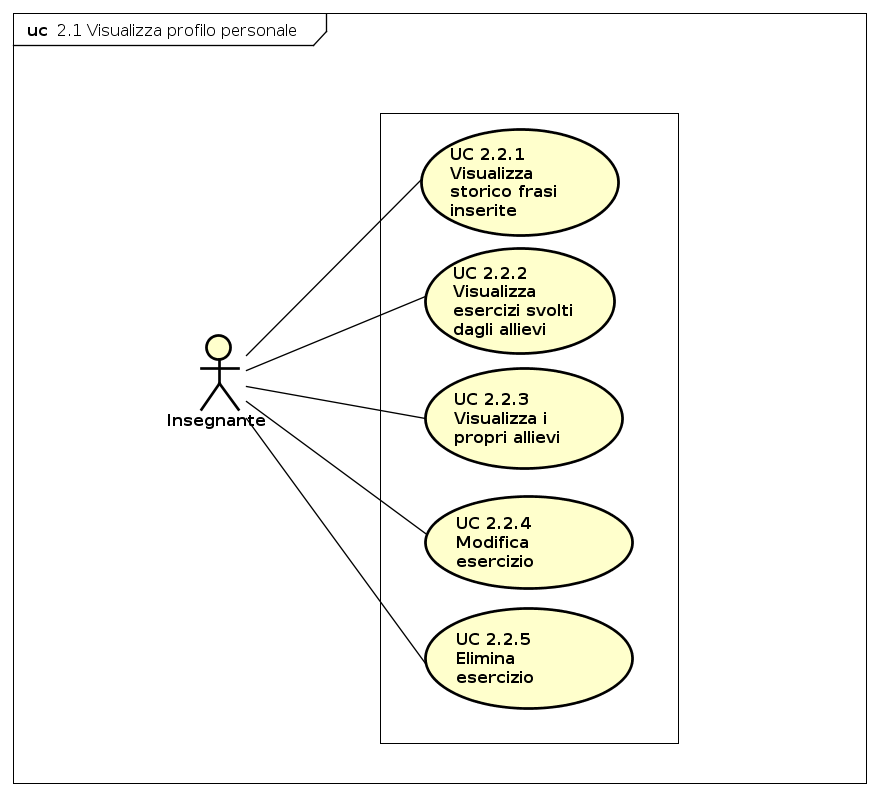
\includegraphics[width=14cm]{img/UC21.png} 
\caption{Caso d'uso UC 2.1}
\end{figure}

\begin{itemize}
	\item[•] \textbf{Attori}: Insegnante;
	\item[•] \textbf{Descrizione}: L’insegnante visualizza il suo profilo personale;

	\item[•] \textbf{Precondizione}: Il sistema offre l’accesso a una dashboard con tutti i dati;

	\item[•] \textbf{Postcondizione}:  Il profilo personale dell’insegnante è aperto;
	\item[•] \textbf{Flusso degli eventi}:
		\begin{enumerate}
			\item UC 2.1.1 Visualizza storico frasi inserite;
			\item UC 2.1.2 Visualizza esercizi svolti dagli allievi;
			\item UC 2.1.3 Visualizza i propri allievi;
			\item UC 2.1.4 Modifica esercizio;
			\item UC 2.1.5 Elimina esercizio.
		\end{enumerate}
\end{itemize}

\subsubsection{UC 2.1.1  Visualizza storico frasi inserite}

\begin{figure}[H]
\centering
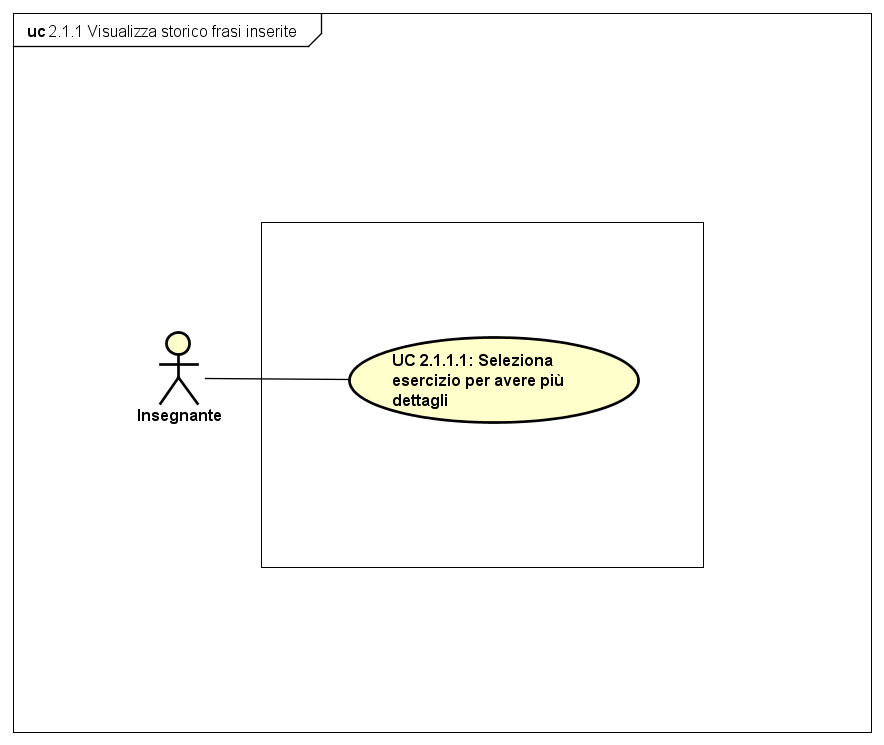
\includegraphics[width=10cm]{img/UC211.png} 
\caption{Caso d'uso UC 2.1.1}
\end{figure}

\begin{itemize}
	\item[•] \textbf{Attori}:  Insegnante	   \item[•] \textbf{Descrizione}: L’insegnante visualizza nel suo profilo personale lo storico delle frasi inserite; 
	\item[•] \textbf{Precondizione}: Il sistema offre la possibilità di visualizzare lo storico delle frasi inserite dall’insegnante;
	\item[•] \textbf{Postcondizione}:  L’insegnante può navigare all’interno della lista di frasi che ha inserito.
	\item[•] \textbf{Flusso degli eventi}:
		\begin{enumerate}
			\item UC 2.1.1.1  Seleziona esercizio per avere più dettagli.
		\end{enumerate}
\end{itemize}

\subsubsection{UC 2.1.1.1 Seleziona esercizio per avere più dettagli}
\begin{itemize}
	\item[•] \textbf{Attori}: Insegnante;
	\item[•] \textbf{Descrizione}:  L’insegnante seleziona dalla lista degli esercizi assegnati un esercizio e ne visualizza i dettagli;
	\item[•] \textbf{Precondizione}: Il sistema offre la possibilità di visualizzare i dettagli relativi ad un esercizio assegnato;
	\item[•] \textbf{Postcondizione}: L’insegnante legge le specifiche dell’esercizio selezionato.
\end{itemize}

\subsubsection{UC 2.1.2  Visualizza esercizi svolti dagli allievi}
\begin{figure}[H]
\centering
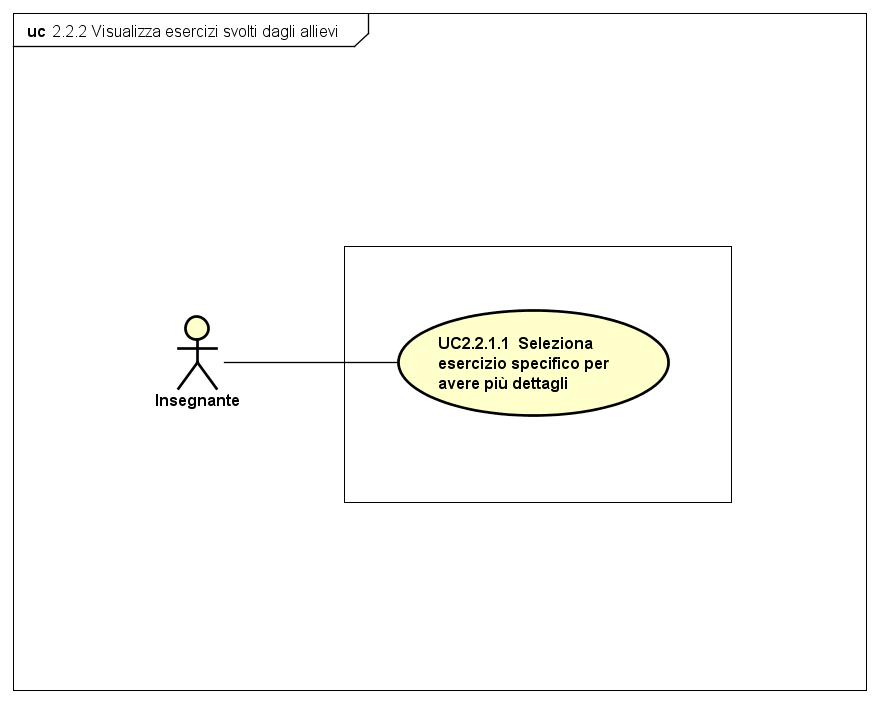
\includegraphics[width=10cm]{img/UC212.png} 
\caption{Caso d'uso UC 2.1.2}
\end{figure}
\begin{itemize}
	\item[•] \textbf{Attori}: Insegnante;
	\item[•] \textbf{Descrizione}:  L’insegnante è nella sezione profilo personale ed entra
		nel registro che conserva gli esercizi svolti dagli allievi;
	\item[•] \textbf{Precondizione}:  L’insegnante ha degli allievi e ha assegnato a loro degli esercizi che sono stati svolti e consegnati;

	\item[•] \textbf{Postcondizione}: L’insegnante può navigare all’interno degli esercizi svolti 
                       svolti dagli allievi; 

	\item[•] \textbf{Flusso degli eventi}:
		\begin{enumerate}
			\item UC 2.1.1.1  Seleziona esercizio specifico per avere più dettagli.	
		\end{enumerate}
\end{itemize}

\subsubsection{UC 2.1.3 Visualizza i propri allievi}

\begin{figure}[H]
\centering
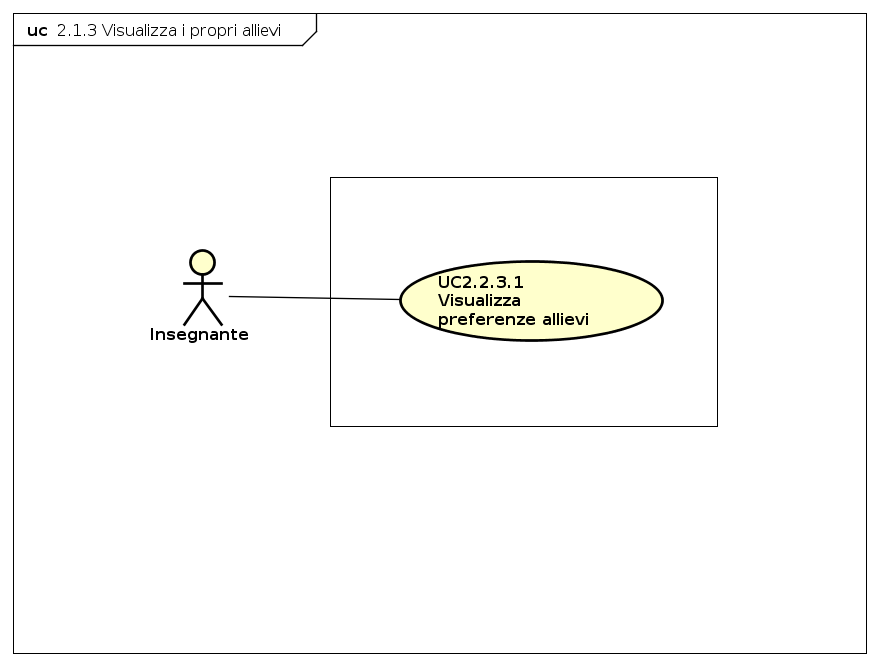
\includegraphics[width=10cm]{img/UC213.png} 
\caption{Caso d'uso UC 2.1.3}
\end{figure}

\begin{itemize}
	\item[•] \textbf{Attori}: Insegnante;
	\item[•] \textbf{Descrizione}: L’insegnante visualizza la lista dei suoi allievi;
	\item[•] \textbf{Precondizione}: Il sistema offre all’insegnante la possibilità di visualizzare la lista dei propri allievi;
	\item[•] \textbf{Postcondizione}: L’insegnante visualizza la lista dei propri allievi;
	\item[•] \textbf{Flusso degli eventi}:
		\begin{enumerate}
			\item UC 2.1.3.1 Visualizza preferenze allievi.
		\end{enumerate}
\end{itemize}

\subsubsection{UC 2.1.3.1 Visualizza preferenze allievi}
\begin{itemize}
	\item[•] \textbf{Attori}: Insegnante;
	\item[•] \textbf{Descrizione}: L’insegnante visualizza nel suo profilo personale il numero di allievi che l'hanno selezionata/o come preferita/o;
	\item[•] \textbf{Precondizione}: Il sistema offre la possibilità di poter segnare un insegnante come preferito;
	\item[•] \textbf{Postcondizione}: L’insegnante può vedere il numero di alunni che l'hanno selezionata/o come preferita/o.
\end{itemize}


\subsubsection{UC 2.1.4 Modifica esercizio}

\begin{figure}[H]
\centering
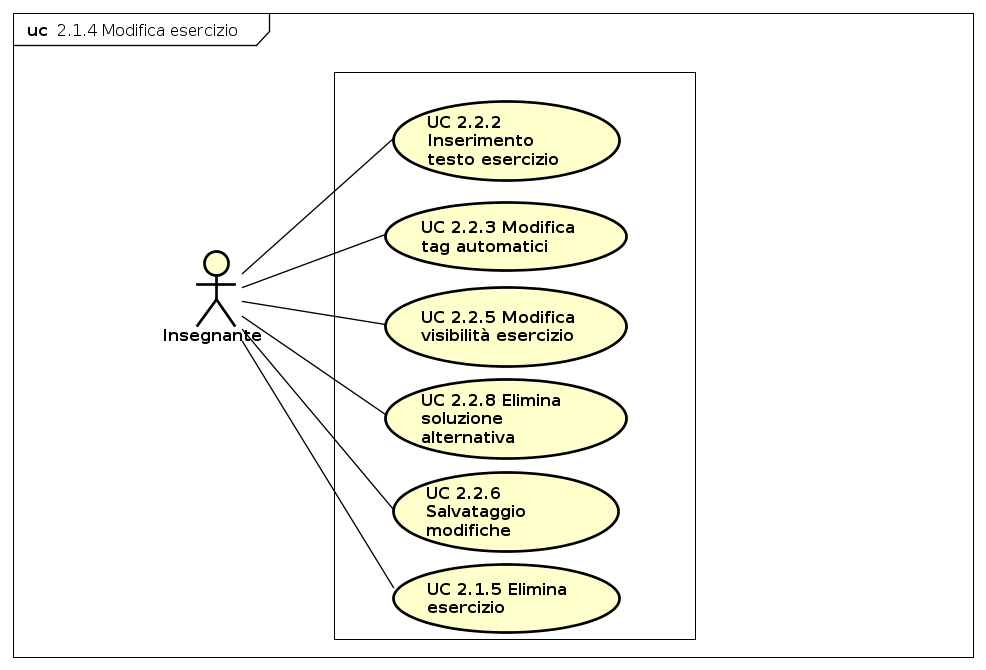
\includegraphics[width=10cm]{img/UC214.png} 
\caption{Caso d'uso UC 2.1.4}
\end{figure}

\begin{itemize}
	\item[•] \textbf{Attori}: Insegnante;
	\item[•] \textbf{Descrizione}: L’insegnante può modificare un esercizio precedentemente inserito;
	\item[•] \textbf{Precondizione}: Il sistema offre la possibilità di modificare il testo, la
				lingua, la visibilità, i {tag}\ped{G} e le soluzioni alternative 
				dell’esercizio;
	\item[•] \textbf{Postcondizione}: L’esercizio è stato modificato;
	\item[•] \textbf{Flusso degli eventi}:
		\begin{enumerate}
			\item UC 2.2.2 Scrittura testo esercizio;
			\item UC 2.2.5 Modifica tag automatici;
			\item UC 2.2.8 Modifica visibilità esercizio.
			\item UC 2.2.9 Salva modifiche
		\end{enumerate}
		    
\end{itemize}   	
	
\subsubsection{UC 2.1.5 Elimina esercizio}
\begin{itemize}
	\item[•] \textbf{Attori}: Insegnante;
	\item[•] \textbf{Descrizione}: L’insegnante elimina un esercizio che è stato assegnato;
	\item[•] \textbf{Precondizione}: Il sistema offre la possibilità di eliminare un esercizio che è stato assegnato;
	\item[•] \textbf{Postcondizione}: L’esercizio assegnato è stato cancellato.
\end{itemize}

%%%%%%%%%%%%%%%%%%%%%%%%%%%%%%%%%%%%%%%%%%%%%%%%%%%%%%%%%%%%%%%%%%%%%%%%%%%%%%%%%%%%%%%%%%%%%%%%%%%%%%%%%%%%%%%%%%

  %%%%%%%%%%%%		PARTE STEFANO		%%%%%%%%%%%%%

%%%%%%%%%%%%%%%%%%%%%%%%%%%%%%%%%%%%%%%%%%%%%%%%%%%%%%%%%%%%%%%%%%%%%%%%%%%%%%%%%%%%%%%%%%%%%%%%%%%%%%%%%%%%%%%%%%



\subsection{UC 2.2 Inserimento di un nuovo esercizio}

\begin{figure}[H]
	\centering
	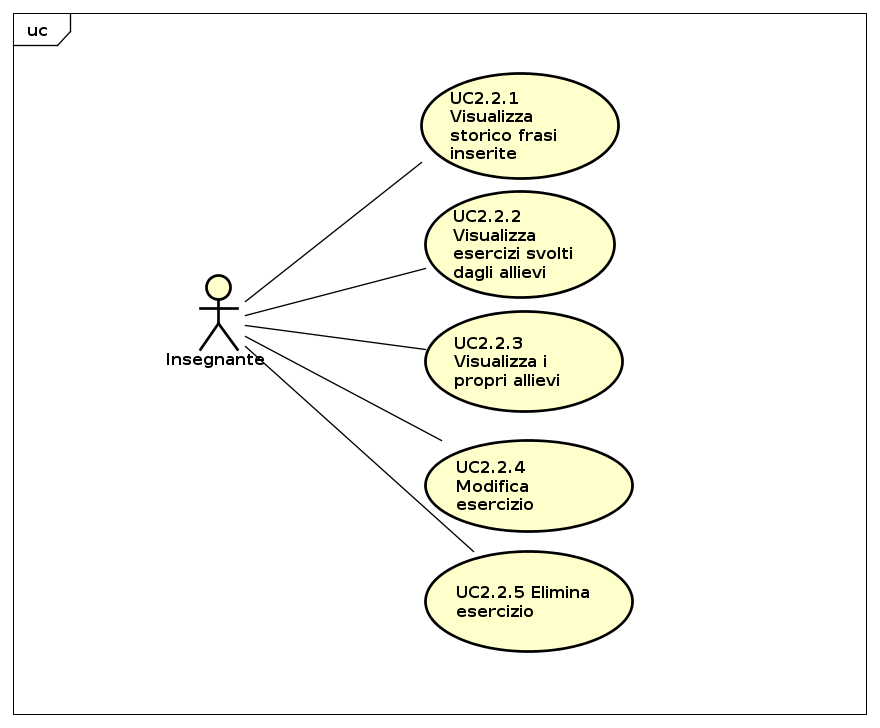
\includegraphics[width=18cm]{img/UC22.png} 
	\caption{Caso d'uso UC 2.2}
\end{figure}

\begin{itemize}
	\item[•] \textbf{Attori}: Insegnante;
	\item[•] \textbf{Descrizione}: L'insegnante aggiunge attraverso una form il testo di un nuovo esercizio;
	\item[•] \textbf{Precondizione}: Il sistema offre la possibilità di aggiungere un esercizio nel sistema;
	\item[•] \textbf{Postcondizione}: Un nuovo esercizio è stato aggiunto;
	\item[•] \textbf{Flusso degli eventi}:
	\begin{enumerate}
		\item UC 2.2.1 Predisporre lingua esercizio;
		\item UC 2.2.2 Scrittura testo esercizio;
		\item UC 2.2.3 Correzione automatica esercizio;
		\item UC 2.2.4 Modifica {tag}\ped{G} automatici;
		\item UC 2.2.5 Inserire più soluzioni;
		\item UC 2.2.6 Modifica visibilità esercizio;
		\item UC 2.2.7 Salva modifiche;
		\item UC 2.2.9 Conferma aggiunta esercizio;
	\end{enumerate}
	\item[•] \textbf{Estensioni}:	
	\begin{enumerate}
		\item UC 2.2.8 Visualizza errori.
	\end{enumerate}
\end{itemize}

\subsubsection{UC 2.2.1 Predisporre lingua esercizio}
\begin{itemize}
	\item[•] \textbf{Attori}: Insegnante;
	\item[•] \textbf{Descrizione}: L'insegnante sceglie la lingua dell’esercizio che vuole scrivere;
	\item[•] \textbf{Precondizione}: Il sistema offre la possibilità di scegliere tra più lingue il testo dell’esercizio;
	\item[•] \textbf{Postcondizione}: La lingua è stata scelta;
\end{itemize}

\subsubsection{UC 2.2.2 Scrittura testo esercizio}

\begin{figure}[H]
	\centering
	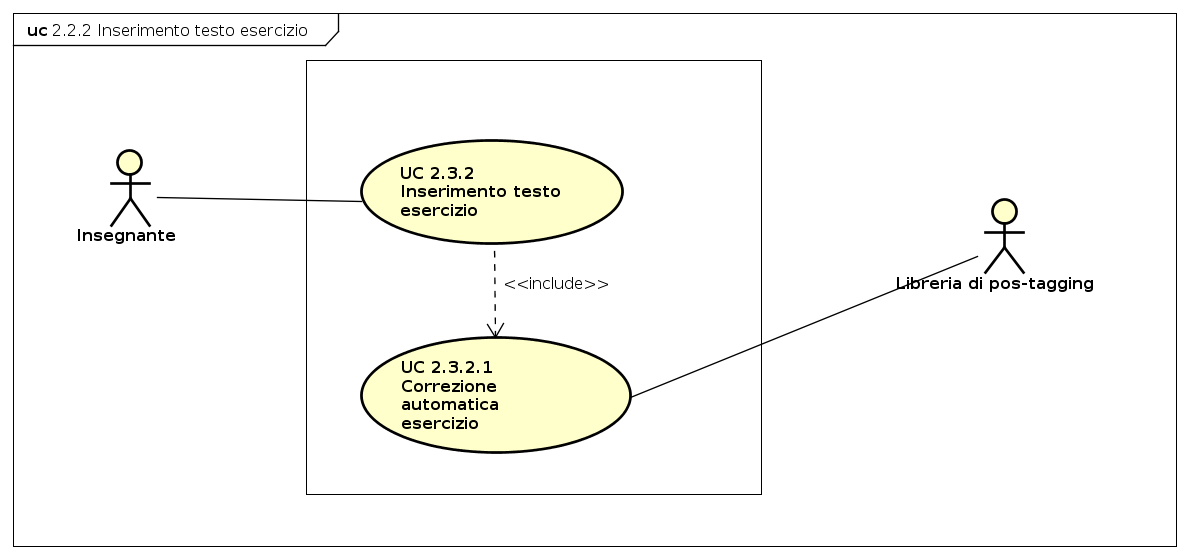
\includegraphics[width=10cm]{img/UC222.png} 
	\caption{Caso d'uso UC 2.2.2}
\end{figure}

\begin{itemize}
	\item[•] \textbf{Attori}: Insegnante;
	\item[•] \textbf{Descrizione}: L'insegnante scrive il testo dell’esercizio;
	\item[•] \textbf{Precondizione}: Il sistema offre la possibilità di scrivere un testo;
	\item[•] \textbf{Postcondizione}: Il testo è stato scritto;
	%\item[•] \textbf{Flusso degli eventi}:
	%\begin{enumerate}
		%\item UC 2.2.2.1 Cancellazione ultimo carattere;
		%\item UC 2.2.2.2 Testo esercizio completato;
	%\end{enumerate}
\end{itemize}


\subsubsection{UC 2.2.3	Correzione automatica esercizio}
\begin{itemize}
	\item[•] \textbf{Attori}: Insegnante e libreria di {PoS-tagging}\ped{G};
	\item[•] \textbf{Descrizione}: L’insegnante genera automaticamente i tag dal testo dell’esercizio attraverso la libreria di PoS-tagging;
\end{itemize}

\subsubsection{UC 2.2.4	Modifica tag automatici}
\begin{itemize}
	\item[•] \textbf{Attori}: Insegnante e libreria di PoS-tagging;
	\item[•] \textbf{Descrizione}: L’insegnante modifica o corregge i tag generati automaticamente;
	\item[•] \textbf{Precondizione}: Il sistema offre la possibilità di modificare i tag generati con la correzione automatica;
	\item[•] \textbf{Postcondizione}: I tag relativi al testo scritto sono stati modificati o corretti;
\end{itemize}

\subsubsection{UC 2.2.5	Inserire più soluzioni}
\begin{itemize}
	\item[•] \textbf{Attori}: Insegnante e libreria di pos-tagging;
	\item[•] \textbf{Descrizione}: L'insegnante inserisce tag alternativi all’esercizio consultando la libreria di PoS-tagging;
	\item[•] \textbf{Precondizione}: Il sistema offre la possibilità di inserire più tag per parola ad esercizio;
	\item[•] \textbf{Postcondizione}: Una soluzione alternativa è stata aggiunta.
\end{itemize}

\subsubsection{UC 2.2.6	Modifica visibilità esercizio}
\begin{itemize}
	\item[•] \textbf{Attori}: Insegnante;
	\item[•] \textbf{Descrizione}: L'insegnante decide chi può visualizzare e svolgere esercizio;
	\item[•] \textbf{Precondizione}: Il sistema offre la possibilità di monitorare visibilità esercizio;
	\item[•] \textbf{Postcondizione}: L’esercizio è stato reso visibile o meno ad un gruppo di utenti.
\end{itemize}

\subsubsection{UC 2.2.7	Salva modifiche}
\begin{itemize}
	\item[•] \textbf{Attori}: Insegnante;
	\item[•] \textbf{Descrizione}: L'insegnante salva esercizio e possibili modifiche;
	\item[•] \textbf{Precondizione}: Il sistema offre la possibilità di salvare gli esercizi creati;
	\item[•] \textbf{Postcondizione}: Un esercizio è stato salvato.
\end{itemize}

\subsubsection{UC 2.2.8 Visualizza errori}
\begin{itemize}
	\item[•] \textbf{Attori}: Insegnante;
	\item[•] \textbf{Descrizione}: L'insegnante visualizza gli errori relativi alla sintassi e la forma dell’esercizio che sta creando;
	\item[•] \textbf{Precondizione}: Il sistema offre la possibilità di visualizzare gli errori effettuati nella scrittura del testo;
	\item[•] \textbf{Postcondizione}: L’esercizio è stato visionato dal sistema, e gli errori sono stati visualizzati.
\end{itemize}

\subsubsection{UC 2.3.1.1 Conferma aggiunta esercizio}
\begin{itemize}
	\item[•] \textbf{Attori}: Insegnante;
	\item[•] \textbf{Descrizione}: L'insegnante aggiunge un esercizio al sistema;
	\item[•] \textbf{Precondizione}: Il sistema offre la possibilità di aggiungere un esercizio;
	\item[•] \textbf{Postcondizione}: L’esercizio è stato aggiunto correttamente al sistema.
\end{itemize}

%\subsection{•}
%\begin{itemize}
%	\item[•] \textbf{Attori}:;
%	\item[•] \textbf{Descrizione}:;
%	\item[•] \textbf{Precondizione}:;
%	\item[•] \textbf{Postcondizione}:;
%	\item[•] \textbf{Flusso degli eventi}:;
%	\begin{enumerate}
%		\item
%		\item
%	\end{enumerate}
%	\item[•] \textbf{Estensioni}:;	
%	\begin{enumerate}
%		\item
%		\item
%	\end{enumerate}
%\end{itemize}





